%%%%%%%%%%%%%%%%%%%%%%%%%%%%%%%%%%%%%%%%%
% baposter Landscape Poster
% LaTeX Template
% Version 1.0 (11/06/13)
%
% baposter Class Created by:
% Brian Amberg (baposter@brian-amberg.de)
%
% This template has been downloaded from:
% http://www.LaTeXTemplates.com
%
% License:
% CC BY-NC-SA 3.0 (http://creativecommons.org/licenses/by-nc-sa/3.0/)
%
%%%%%%%%%%%%%%%%%%%%%%%%%%%%%%%%%%%%%%%%%

%----------------------------------------------------------------------------------------
%	PACKAGES AND OTHER DOCUMENT CONFIGURATIONS
%----------------------------------------------------------------------------------------

\documentclass[portrait,a0paper,fontscale=0.285]{baposter} % Adjust the font scale/size here

\usepackage{graphicx} % Required for including images
\graphicspath{{figures/}} % Directory in which figures are stored

\usepackage{amsmath} % For typesetting math
\usepackage{amssymb} % Adds new symbols to be used in math mode

\usepackage{booktabs} % Top and bottom rules for tables
\usepackage{enumitem} % Used to reduce itemize/enumerate spacing
\usepackage{palatino} % Use the Palatino font
\usepackage[font=small,labelfont=bf]{caption} % Required for specifying captions to tables and figures
\usepackage{grffile} % can use other graphics extensions (e.g. doesn't error for example.0.1.png)
\usepackage{caption}

\usepackage{multicol} % Required for multiple columns
\usepackage{url} % For references which have website URLs
\setlength{\columnsep}{1.5em} % Slightly increase the space between columns
\setlength{\columnseprule}{0mm} % No horizontal rule between columns

\usepackage{tikz} % Required for flow chart
\usetikzlibrary{shapes,arrows} % Tikz libraries required for the flow chart in the template

\usepackage{array}
\newcolumntype{P}[1]{>{\centering\arraybackslash\vspace{-2mm}}p{#1}} % P-alignment in tables ensures both vertical and horizontal centered.

\newcommand{\compresslist}{ % Define a command to reduce spacing within itemize/enumerate environments, this is used right after \begin{itemize} or \begin{enumerate}
\setlength{\itemsep}{1pt}
\setlength{\parskip}{0pt}
\setlength{\parsep}{0pt}
}

%\definecolor{lightblue}{rgb}{0.145,0.6666,1} % Defines the color used for content box headers
\definecolor{lightblue}{rgb}{1,0.3333,0.3333} %not very 'light blue'

\begin{document}

\begin{poster}
{
headerborder=closed, % Adds a border around the header of content boxes
colspacing=1em, % Column spacing
bgColorOne=white, % Background color for the gradient on the left side of the poster
bgColorTwo=white, % Background color for the gradient on the right side of the poster
borderColor=lightblue, % Border color
headerColorOne=black, % Background color for the header in the content boxes (left side)
headerColorTwo=lightblue, % Background color for the header in the content boxes (right side)
headerFontColor=white, % Text color for the header text in the content boxes
boxColorOne=white, % Background color of the content boxes
textborder=roundedleft, % Format of the border around content boxes, can be: none, bars, coils, triangles, rectangle, rounded, roundedsmall, roundedright or faded
eyecatcher=true, % Set to false for ignoring the left logo in the title and move the title left
headerheight=0.1\textheight, % Height of the header
headershape=roundedright, % Specify the rounded corner in the content box headers, can be: rectangle, small-rounded, roundedright, roundedleft or rounded
headerfont=\Large\bf\textsc, % Large, bold and sans serif font in the headers of content boxes
%textfont={\setlength{\parindent}{1.5em}}, % Uncomment for paragraph indentation
linewidth=2pt % Width of the border lines around content boxes
}
%----------------------------------------------------------------------------------------
%	TITLE SECTION 
%----------------------------------------------------------------------------------------
%
{
\includegraphics[height=3em]{IITlogo.png}} % First university/lab logo on the left
{\bf\huge{\hspace{-1.5in}Hybrid Methods for Simulation \\ \hspace{-1.5in}of Muon Ionization Cooling Channels}\vspace{0.1em}} % Poster title
{{ \large{\hspace{-1.5in}J. Kunz, P. Snopok$^1$ \hspace{12pt} Illinois Institute of Technology \\\hspace{-1.5in}M. Berz, K. Makino \hspace{12pt}Michigan State University \\\hspace{-1.5in}$^1$ also at Fermi National Accelerator Laboratory \vspace{-0.4em}}}}
{
\includegraphics[height=6em]{MAPlogo.png}} % Second university/lab logo on the right

%----------------------------------------------------------------------------------------
%	MICE Layout
%----------------------------------------------------------------------------------------

\headerbox{Muon Ionization Cooling Experiment (MICE) Layout}{name=mice,column=0,row=0,span=2}{
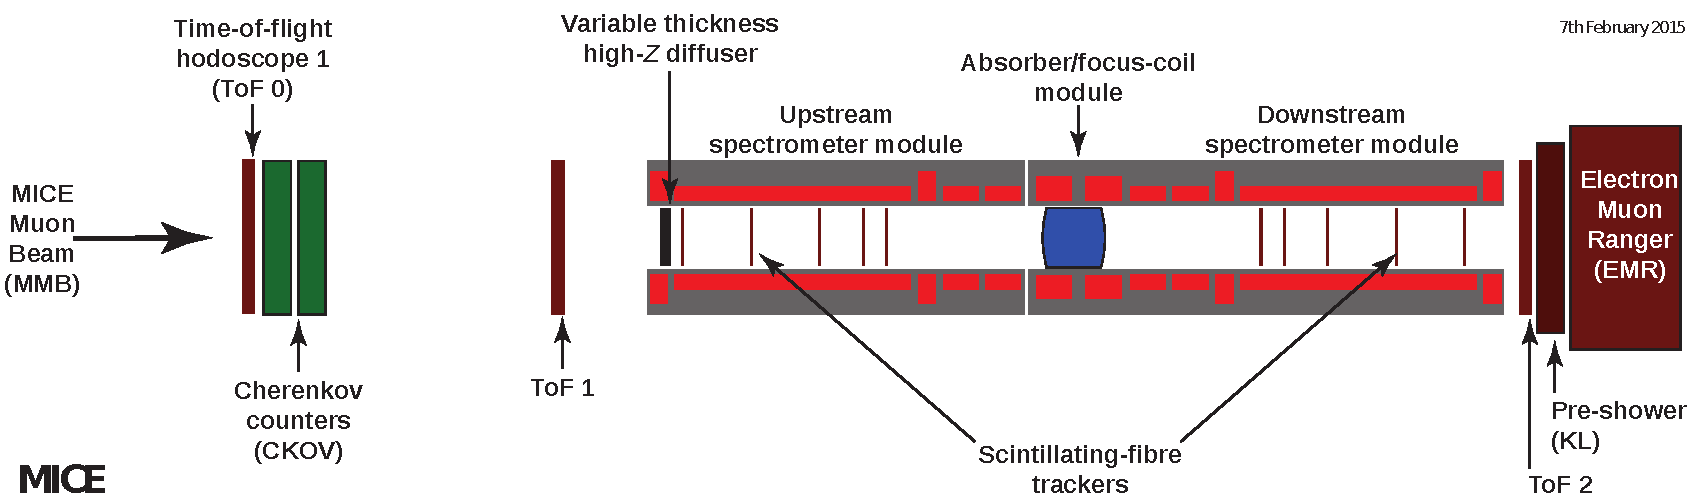
\includegraphics[width=\textwidth]{mice}
}

%----------------------------------------------------------------------------------------
%	Absorbers
%----------------------------------------------------------------------------------------

\headerbox{Absorbers}{name=absorbers,column=0,row=1,below=mice}
{

Recently \cite{ipac2015}, COSY Infinity \cite{cosy} has been outfitted with new simulations tools for matter-dominated lattices, with the application of cooling absorbers as the motivation. Some of these results are reproduced here.
\\

Excellent agreement has been achieved between COSY, G4Beamline \cite{g4bl}, and ICOOL \cite{icool} for pencil beams of $p =$ (100, 200, 300, 400) MeV/\textit{c} through liquid hydrogen absorbers of lengths $L =$ (1, 10, 100) mm. Shown below is an example of this agreement at typical cooling cell parameters: $p =$ 200 MeV/\textit{c}, $L =$ 100 mm.\\
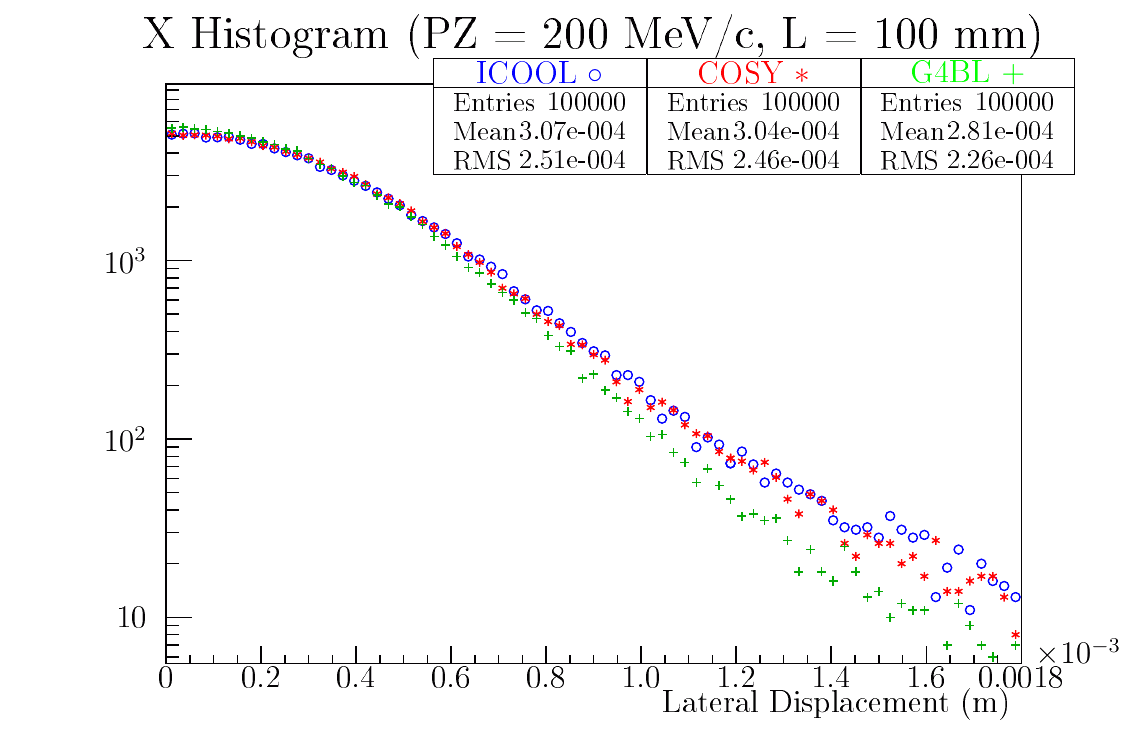
\includegraphics[width=0.49\textwidth]{Figures/LH.X.200.100.png} 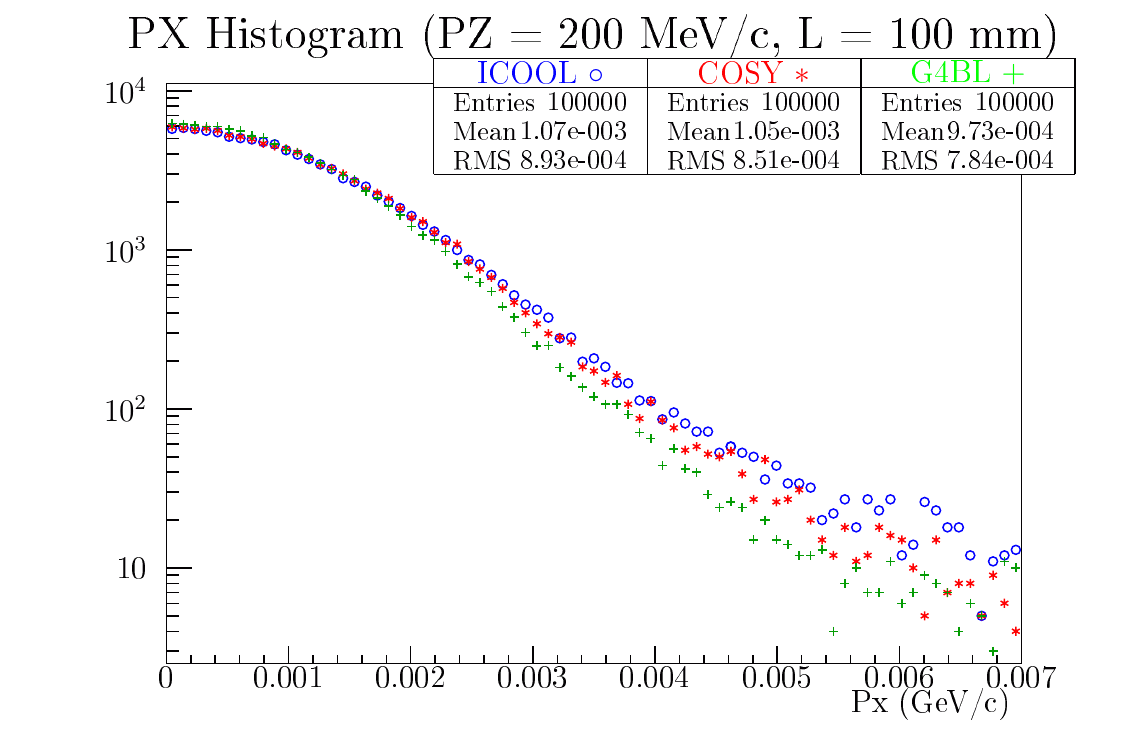
\includegraphics[width=0.49\textwidth]{Figures/LH.PX.200.100.png}
\begin{center} 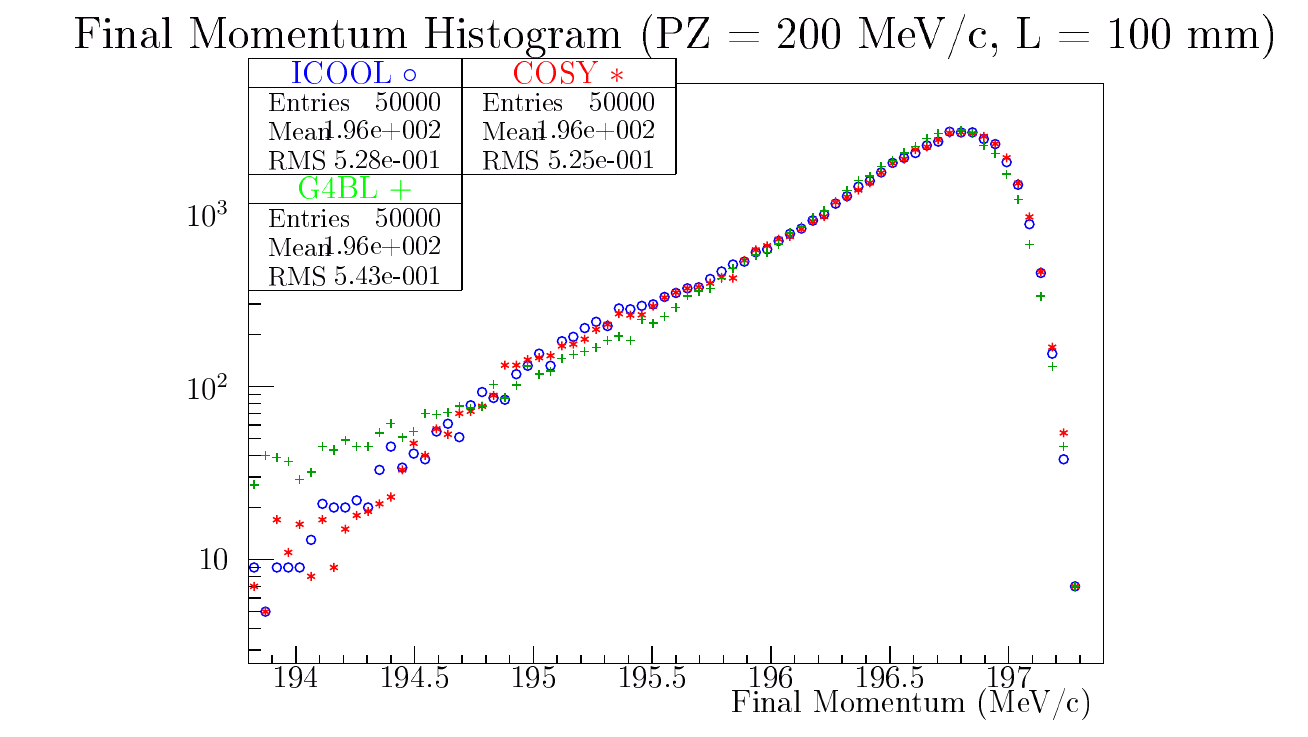
\includegraphics[width=0.5\textwidth]{Figures/LH.strag.200.100.png} \end{center}

Moreover, COSY has been compared to the experimental results of the Muon Scattering Experiment \cite{muscat}. Agreement has been shown for Be @ 3.73 mm, LH @ 159 mm, and LH @ 109 mm, with the last result reproduced below.

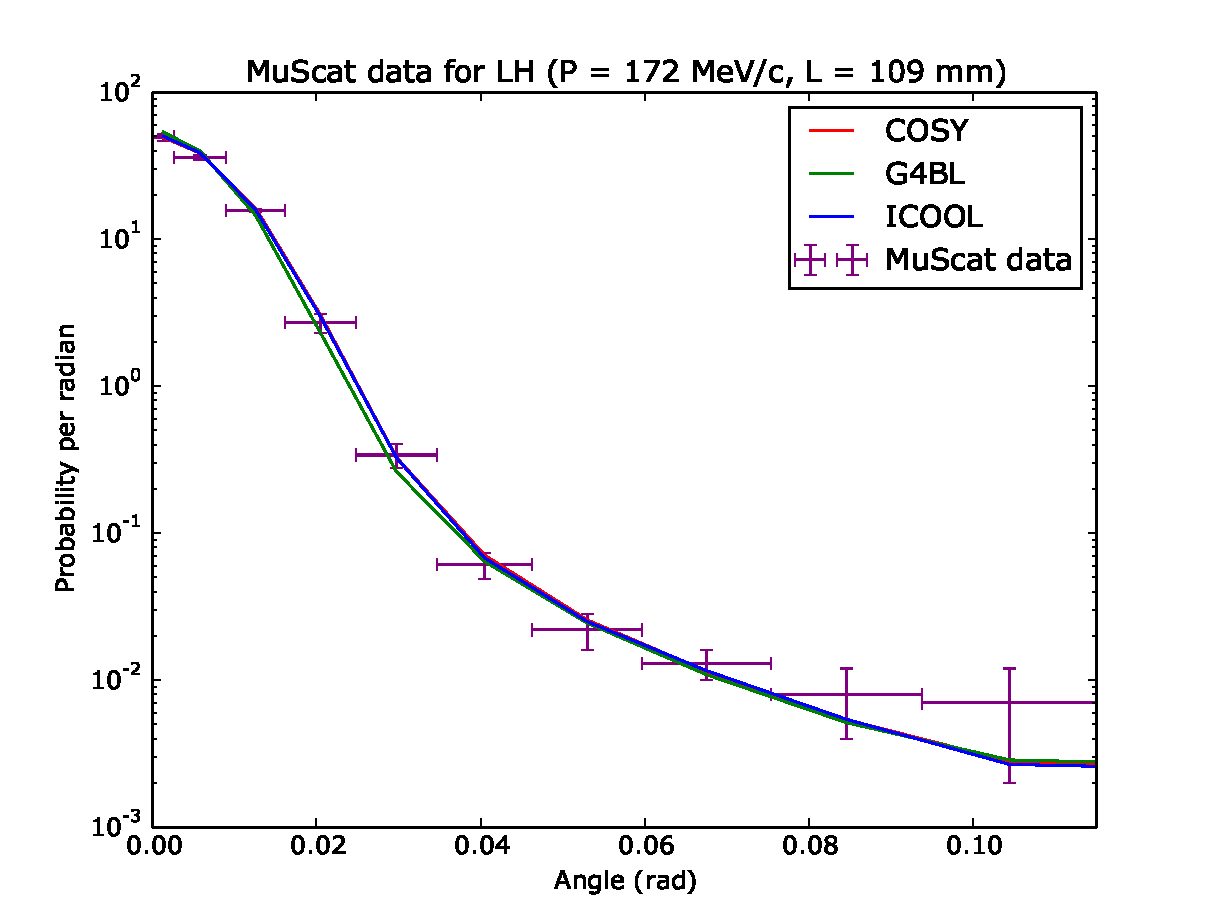
\includegraphics[width=\textwidth]{Figures/172.109.muscat.pdf}
}

%----------------------------------------------------------------------------------------
% 	Magnetic Coils
%----------------------------------------------------------------------------------------

\headerbox{Magnetic coils}{name=coils,column=1,row=1,below=mice}
{
For compact magnetic solenoids, COSY uses the procedure \texttt{CMSTP} (Compact Magnetic Solenoid Thick Piece). Twelve ``test coils" (see table of coil parameters) were benchmarked against G4Beamline's \texttt{coil} and \texttt{solenoid} combination routines. A single cell consisted of two postive current coils at z = 175, 325 mm and two negative current coils at z = 675, 825 mm. The initial distribution was a grid of muons with transverse ranges x = (-100, 100) mm, y = (-100, 100) mm. The result can be seen below.
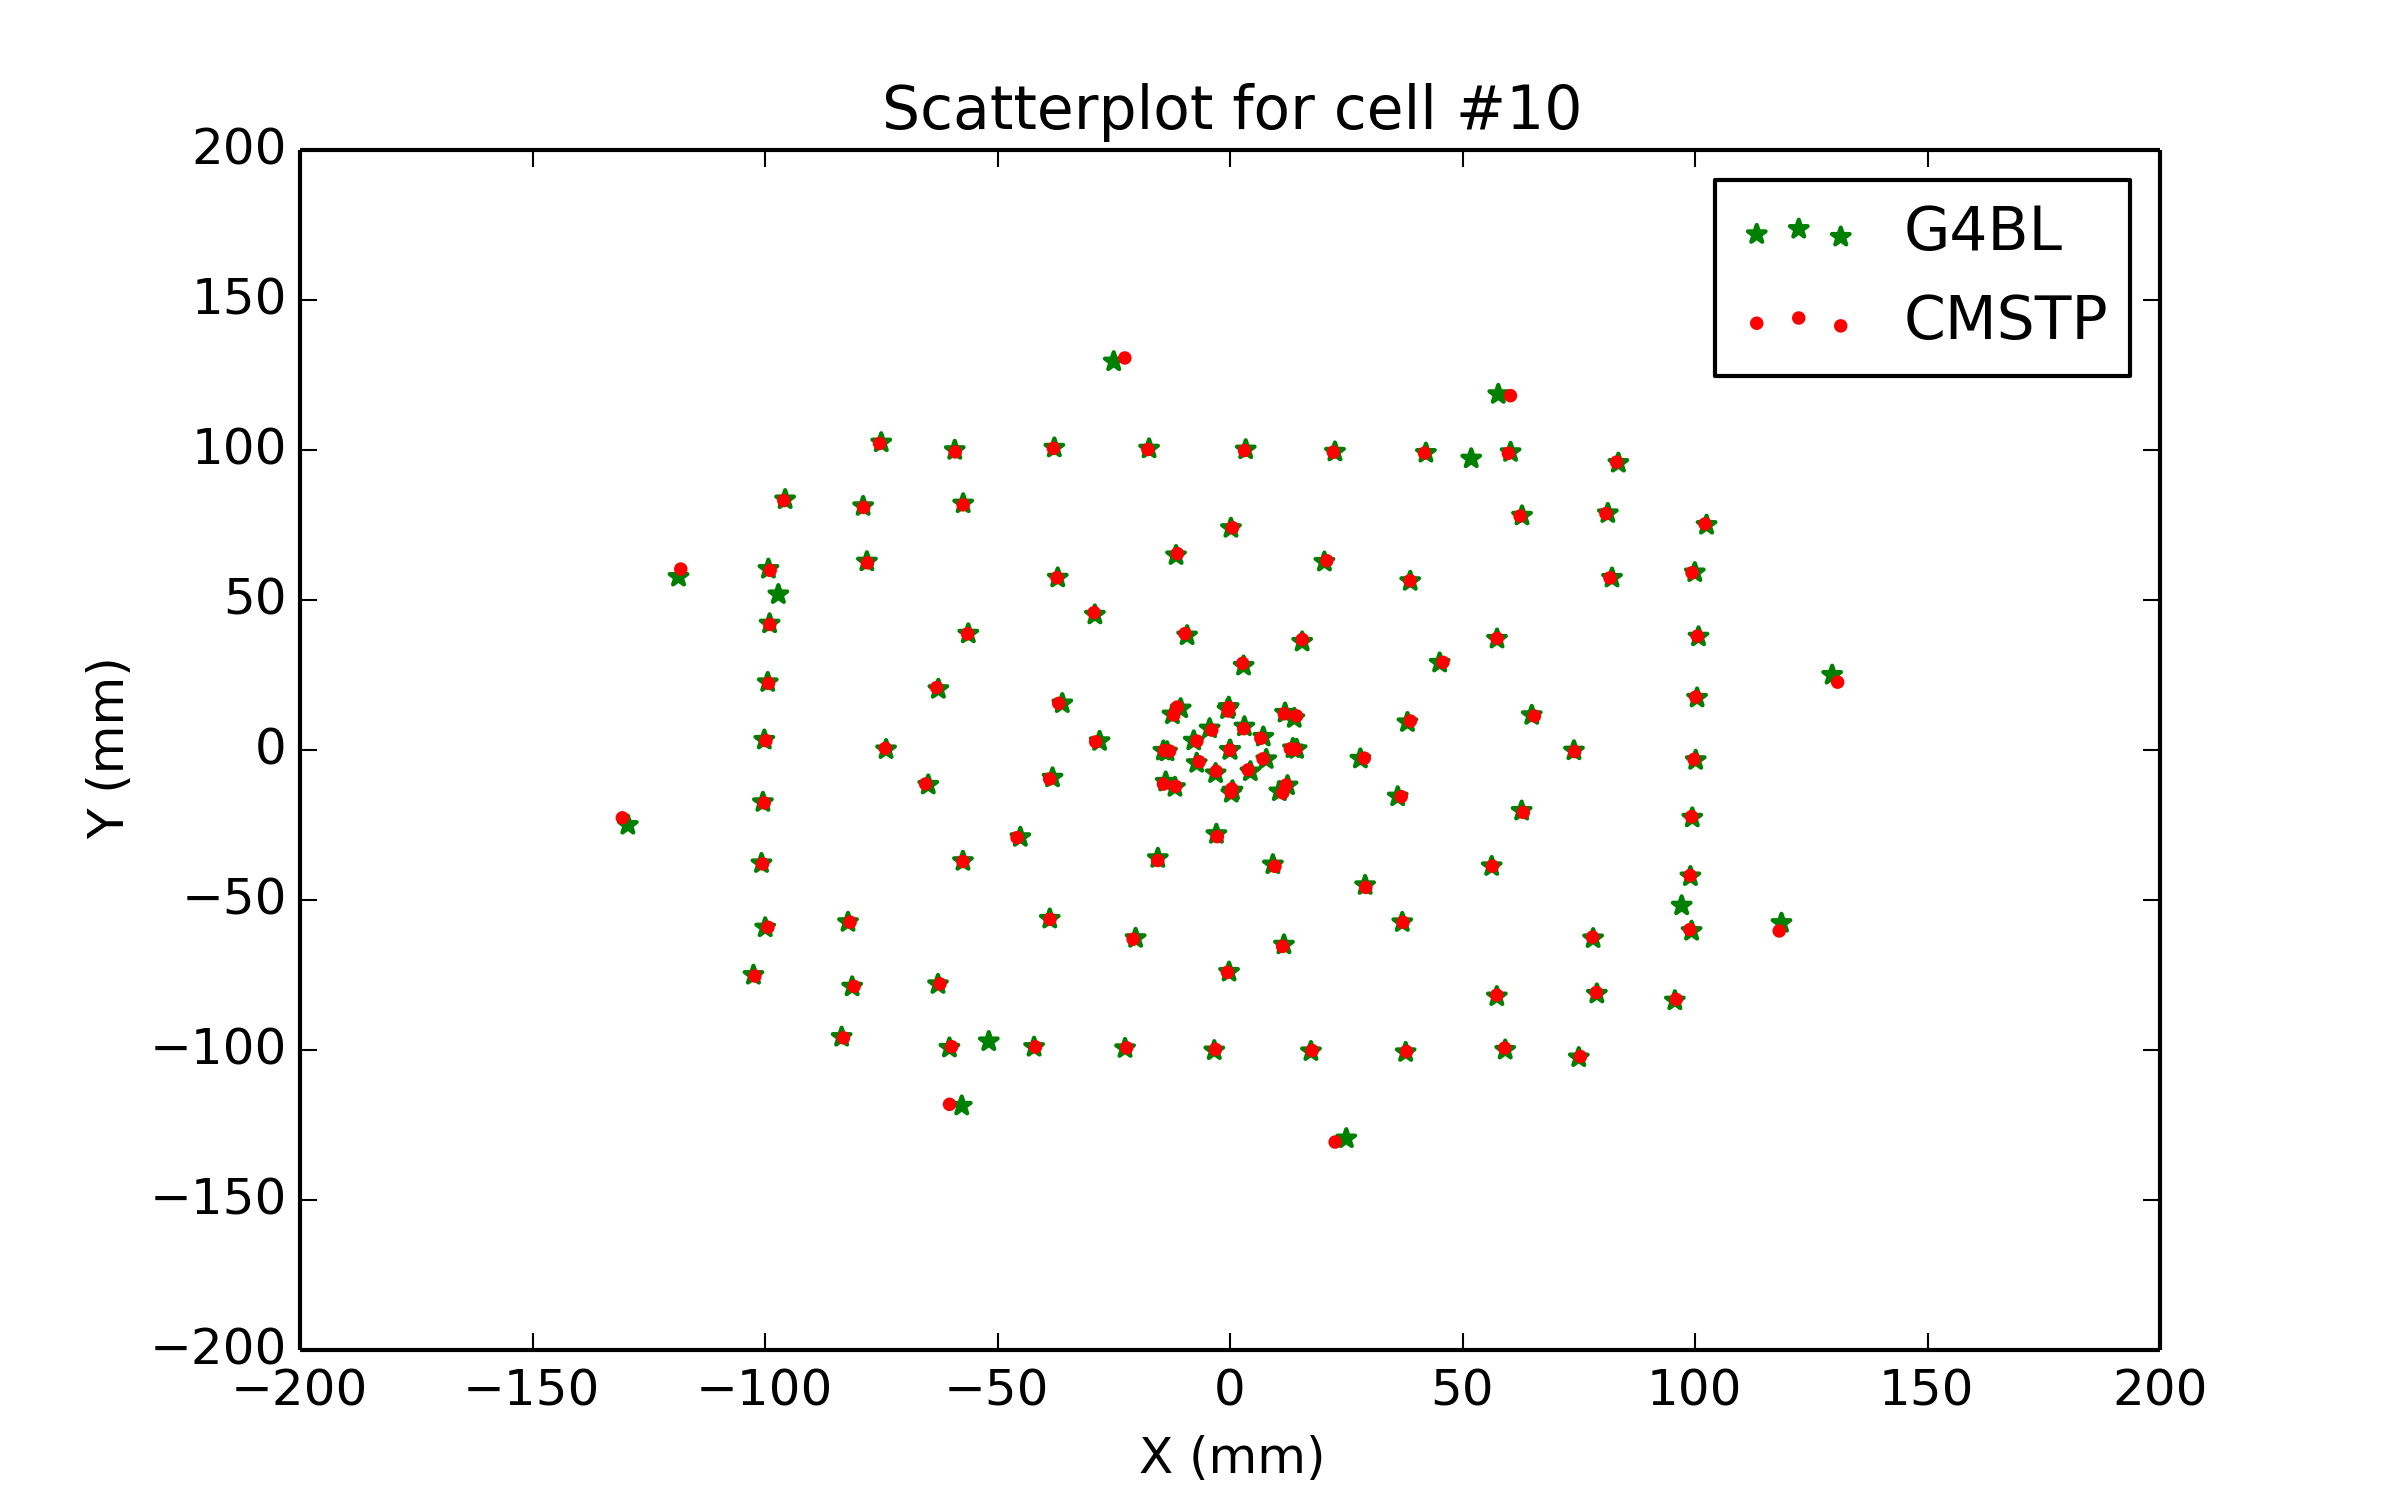
\includegraphics[width=\textwidth]{Figures/grid_cell_10.png}

\begin{center} 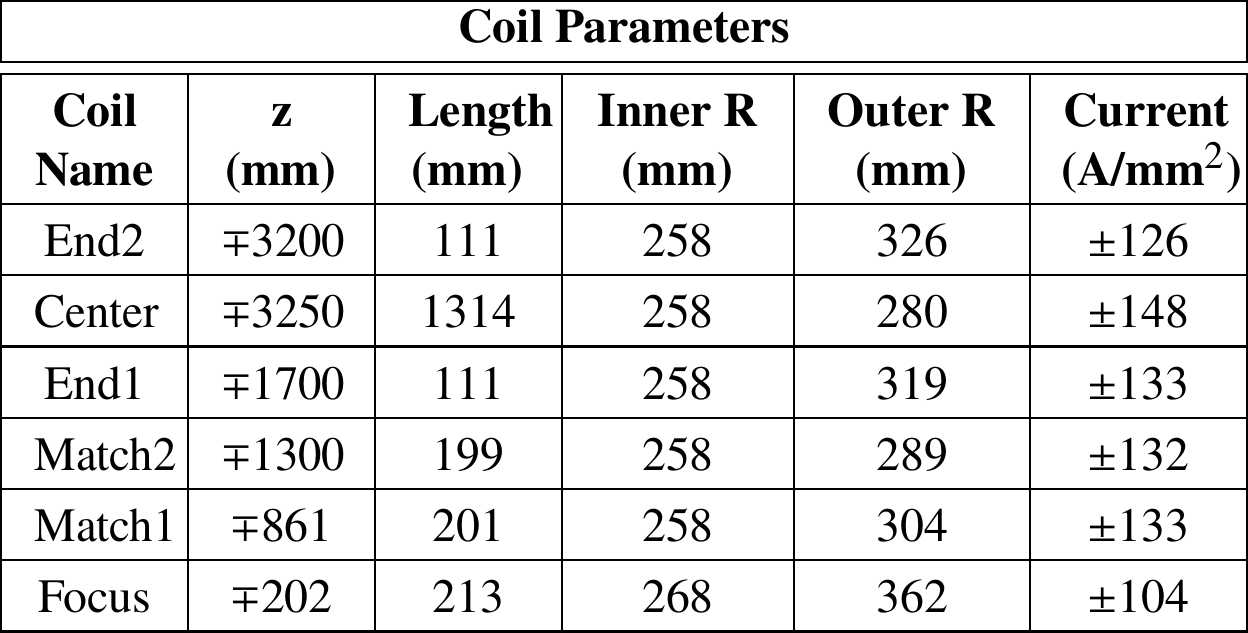
\includegraphics[width=0.95\textwidth]{Figures/coiltable} \end{center}
}

%----------------------------------------------------------------------------------------
%	MICE Cell
%----------------------------------------------------------------------------------------

\headerbox{The MICE cell}{name=micecell,column=2,row=0}
{
MICE was simulated in-parts by COSY and G4Beamline. The initial distribution can be seen in the table below, along with the results of these separate simualtions.
\begin{center} 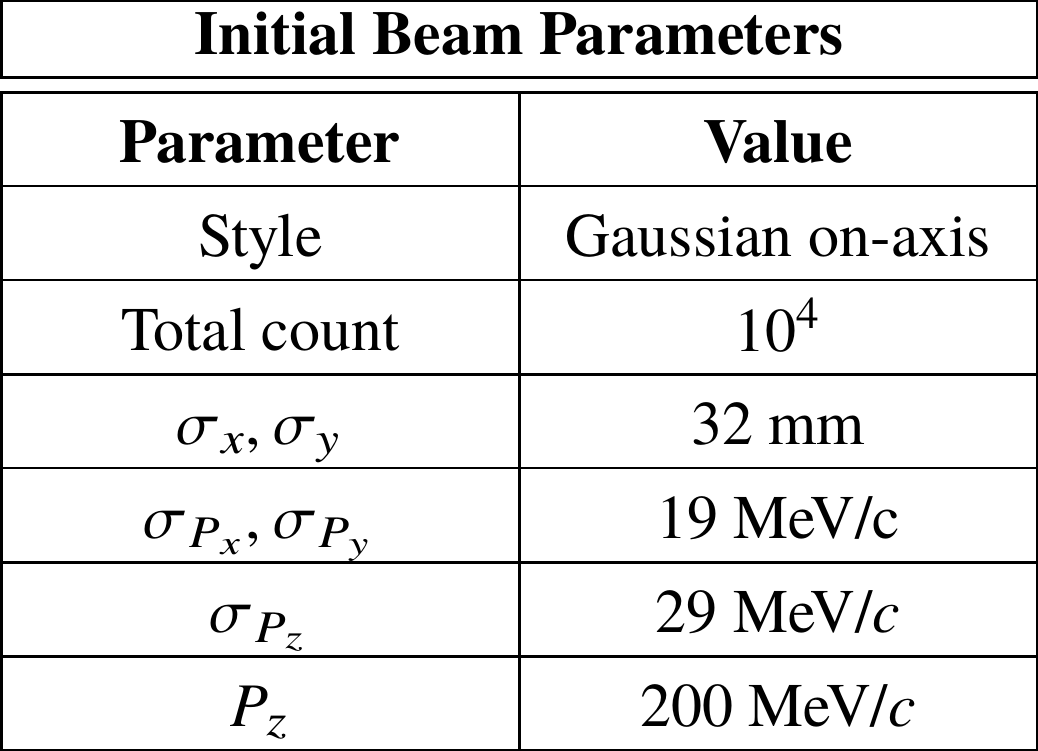
\includegraphics[width=0.75\textwidth]{Figures/initial_distribution_table} \end{center}
The absorber was a cylindrical lithium hydride block of 65 mm.\\
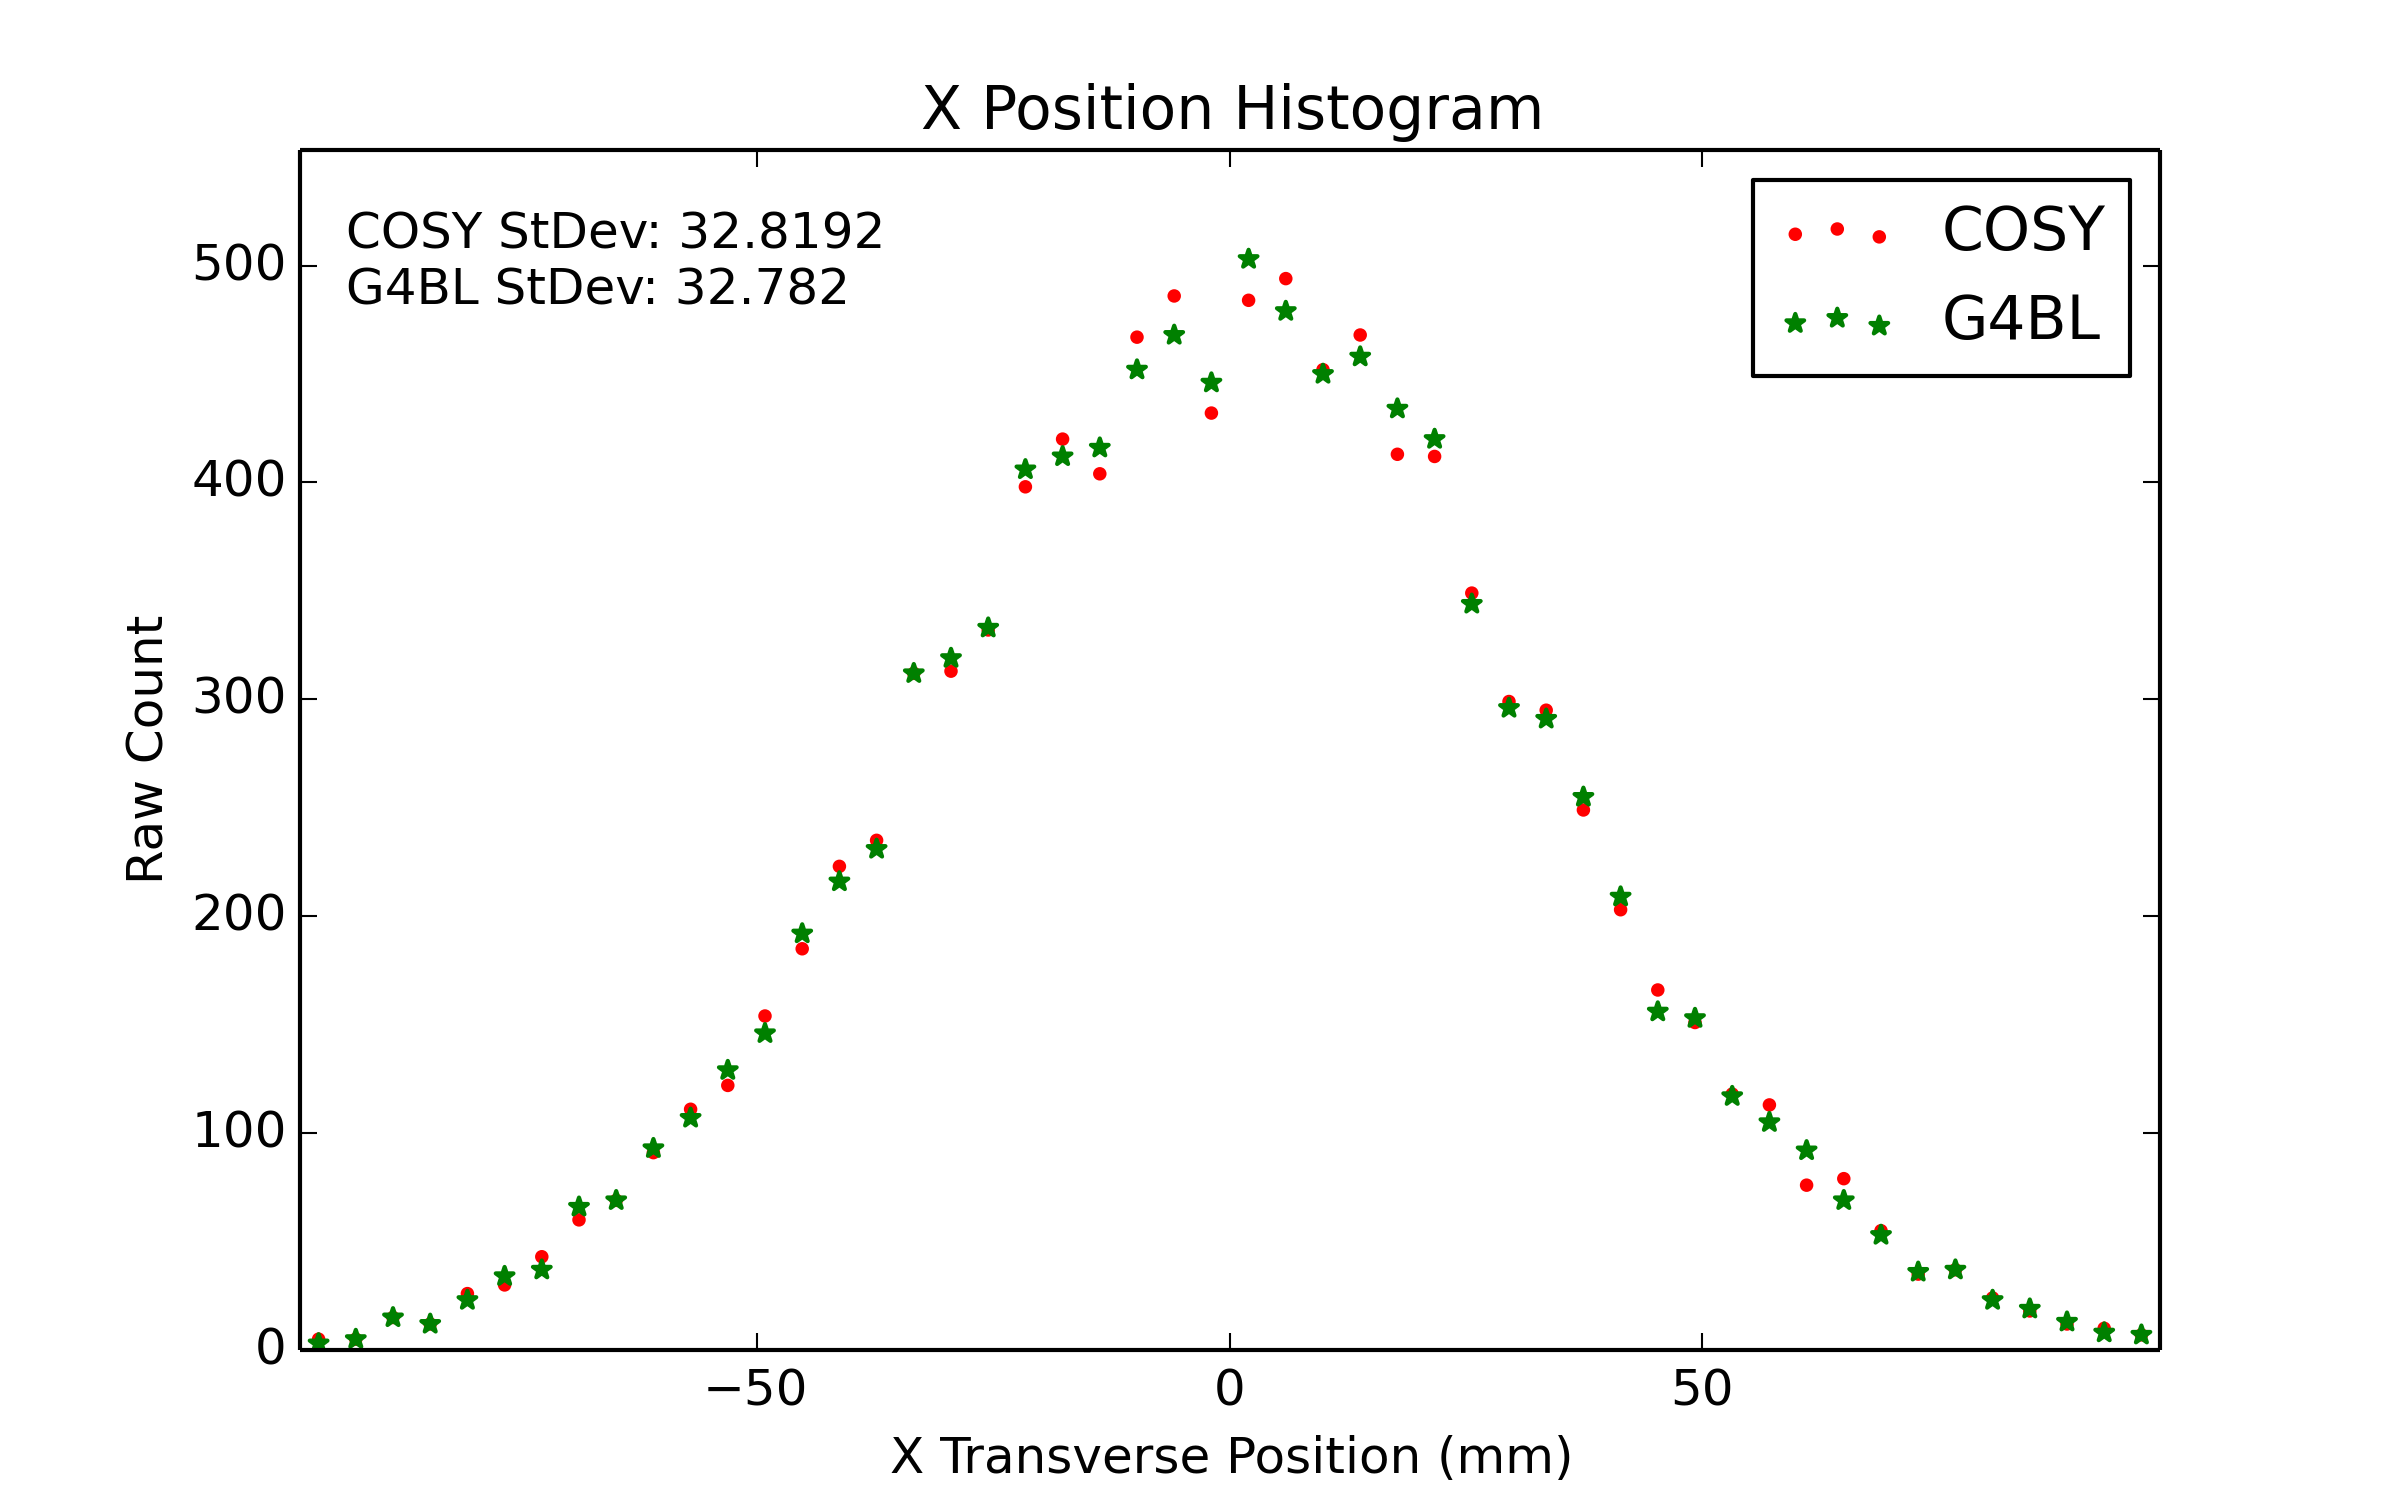
\includegraphics[width=0.5\textwidth]{Figures/wedge tests (LiH)/xposition}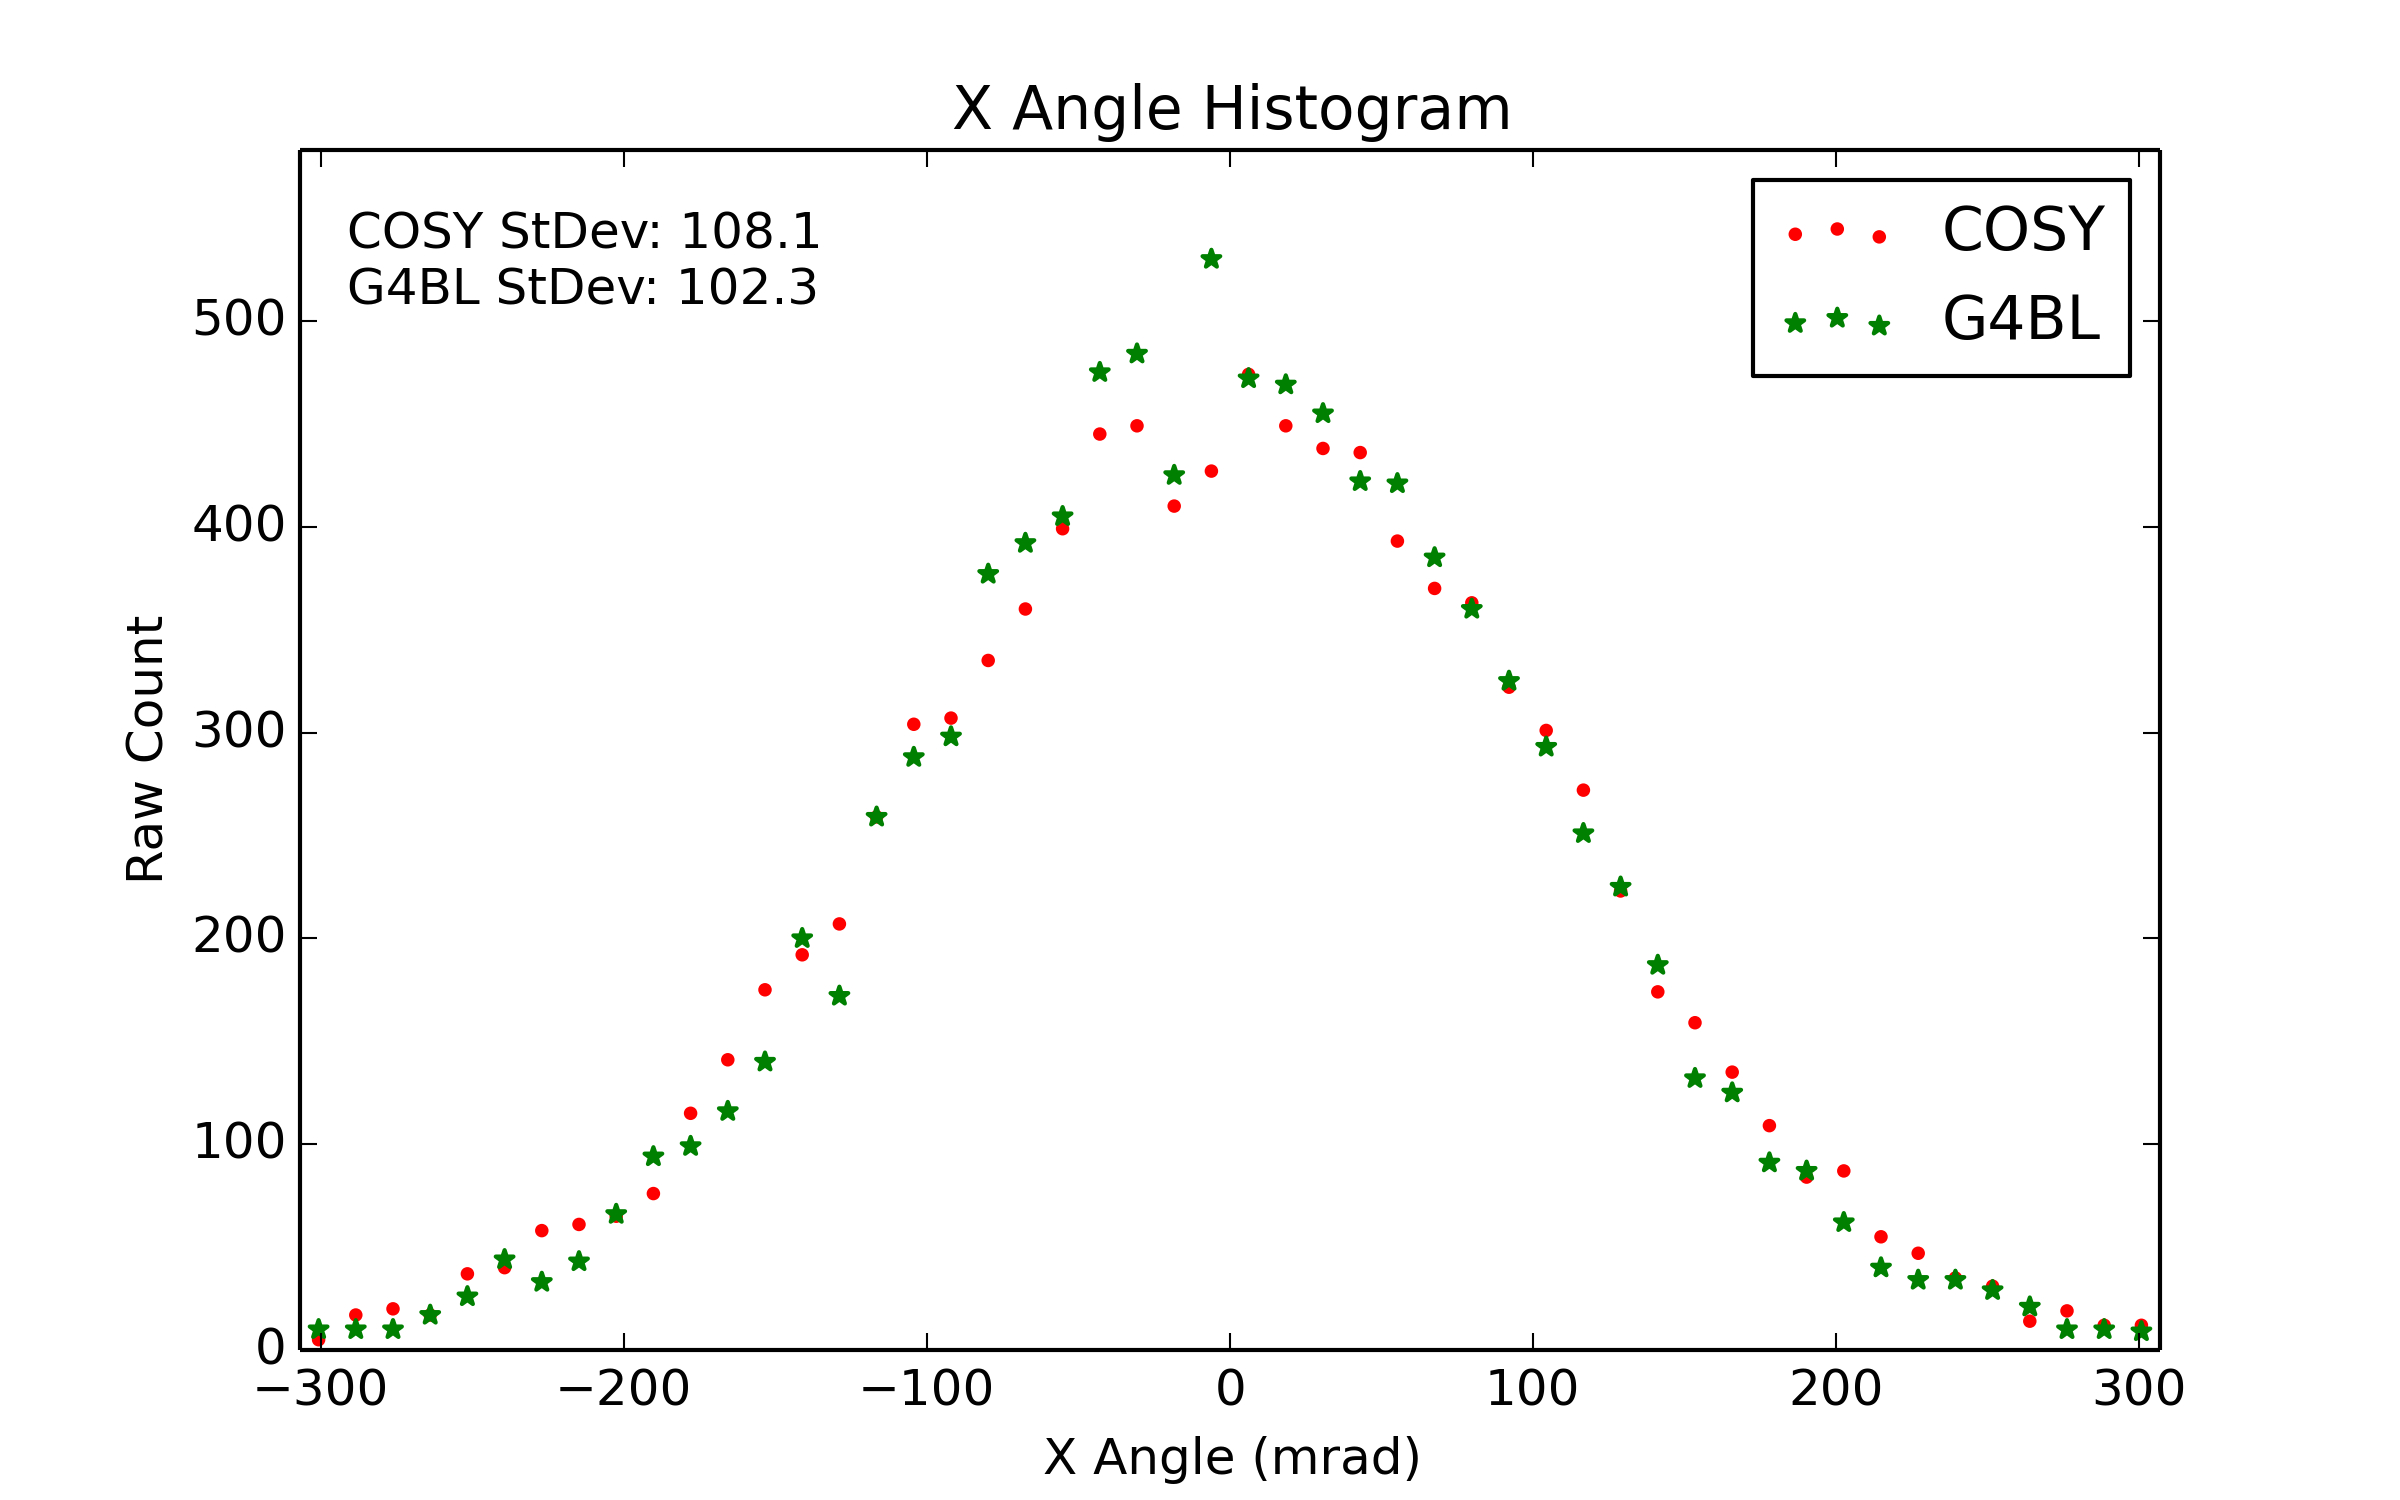
\includegraphics[width=0.5\textwidth]{Figures/wedge tests (LiH)/xangle}
\begin{center} 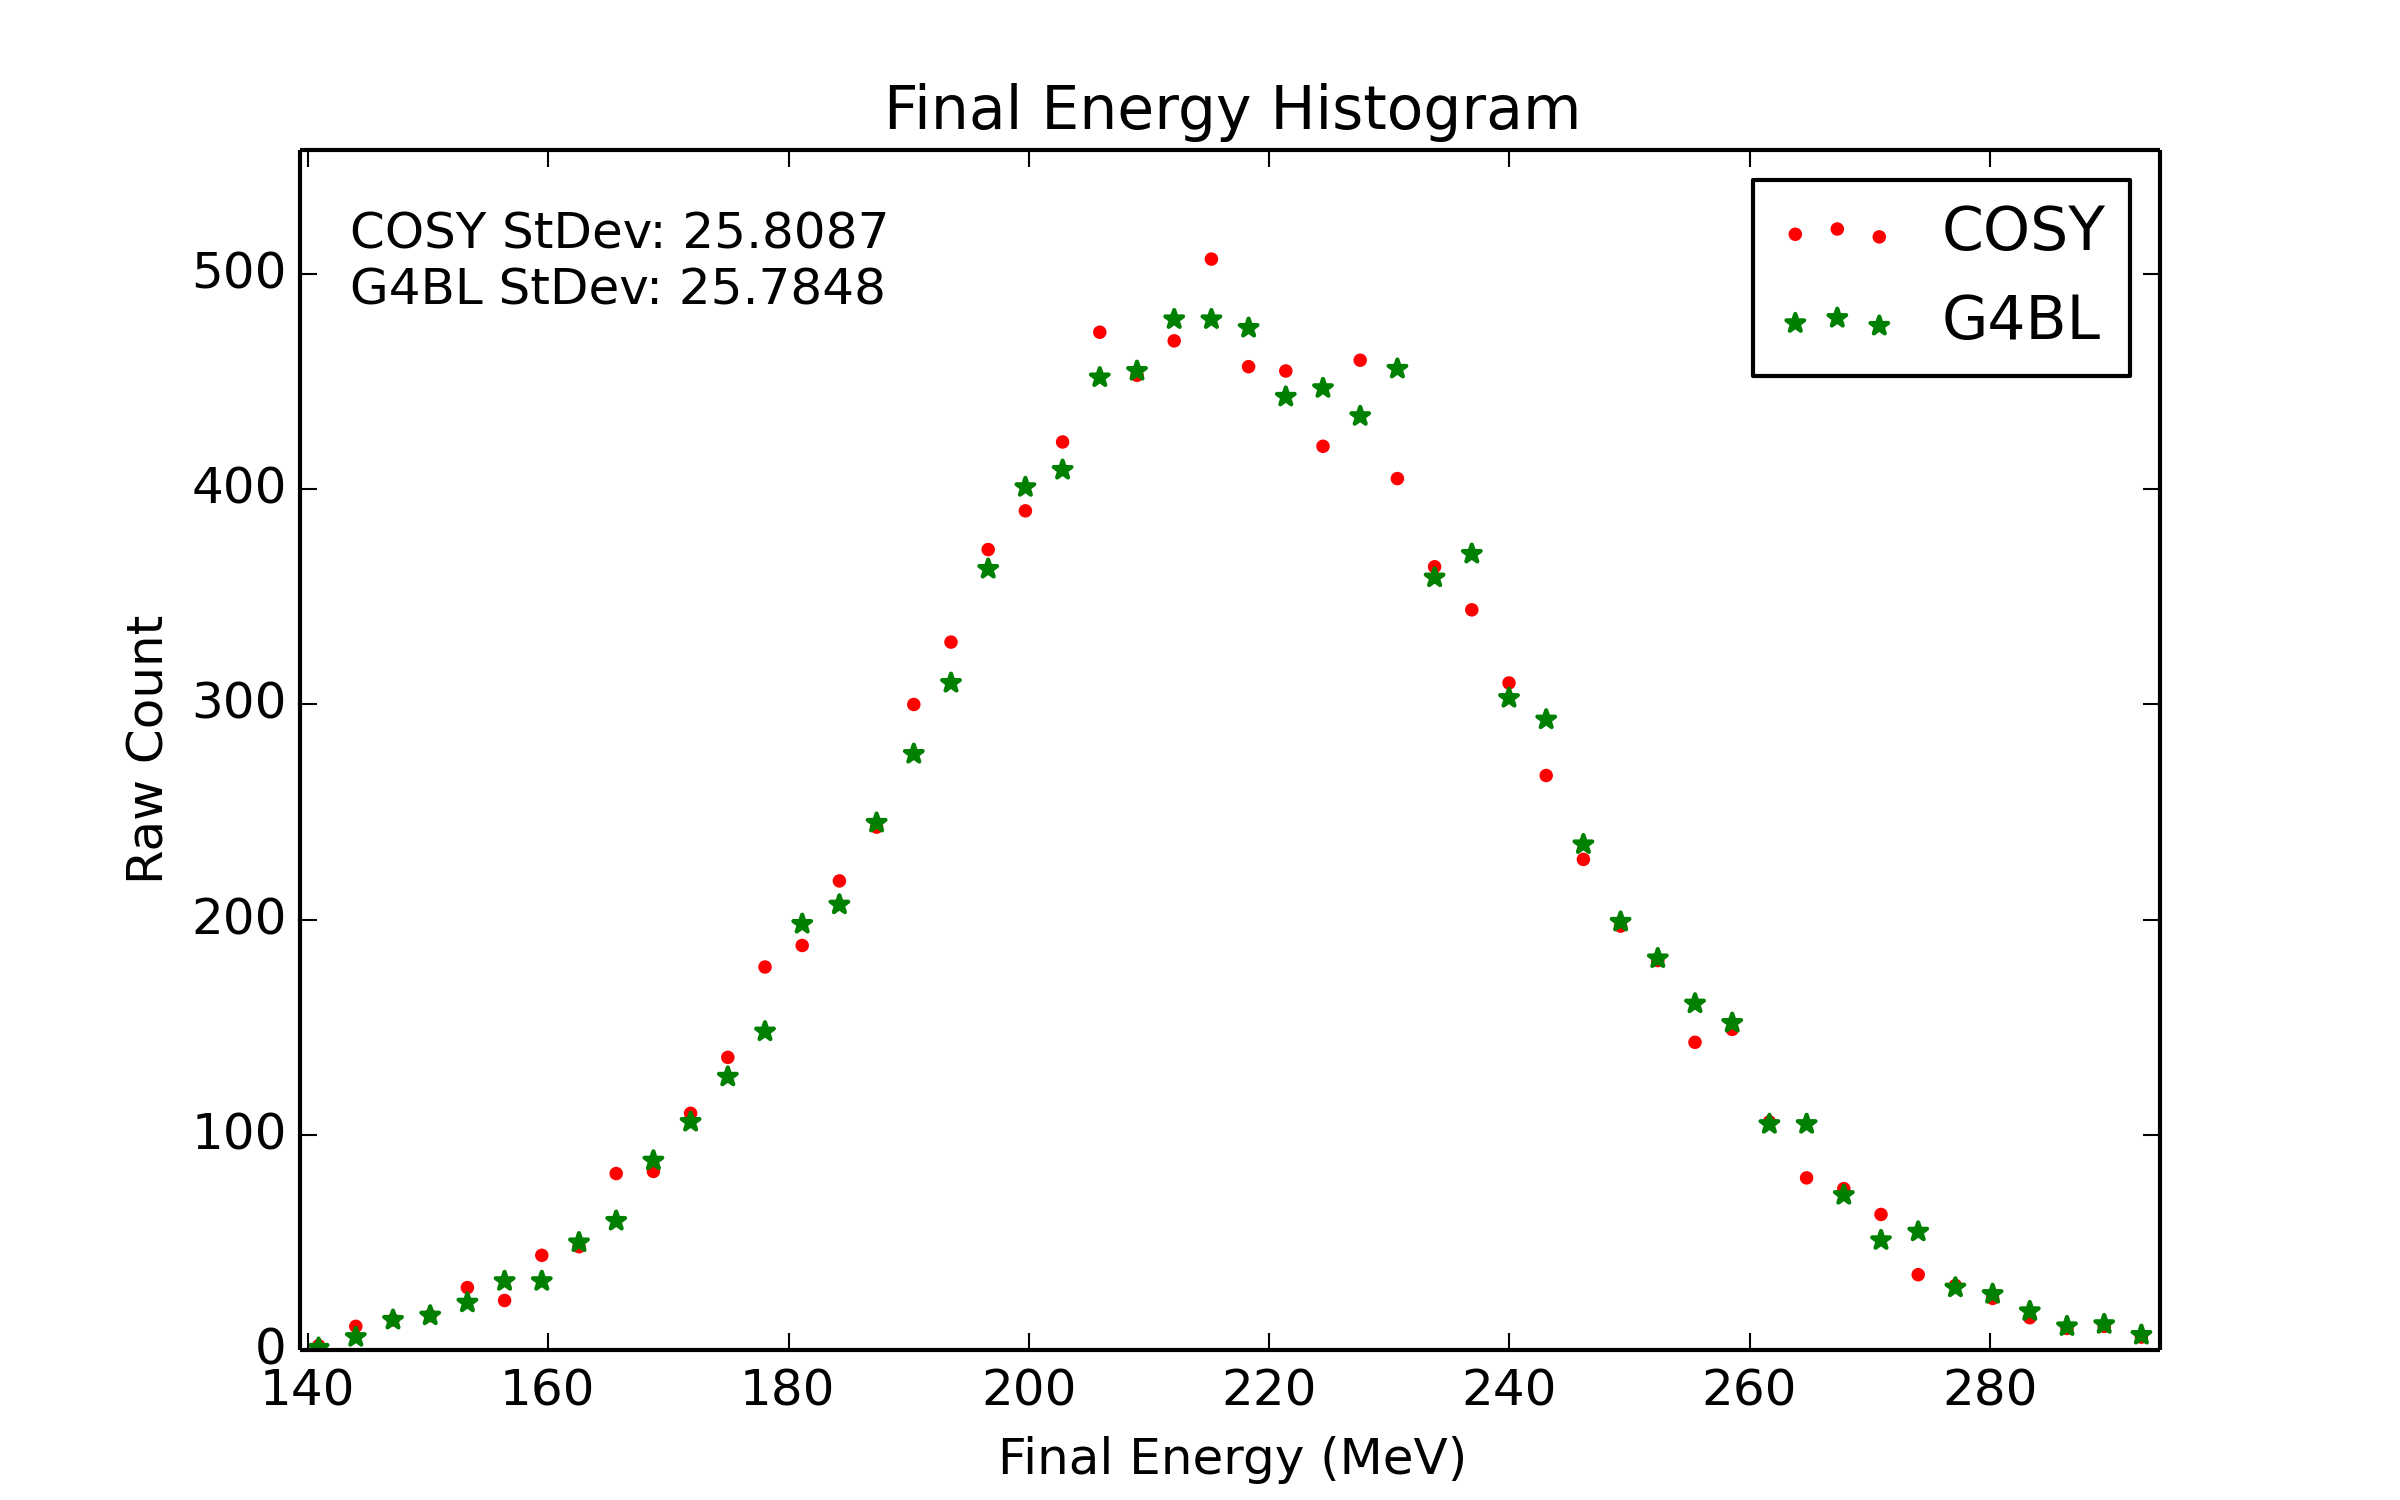
\includegraphics[width=0.5\textwidth]{Figures/wedge tests (LiH)/energy} \end{center}
The coils (as seen in the MICE layout figure) were simulated to and from the scintillating-fibre trackers.\\
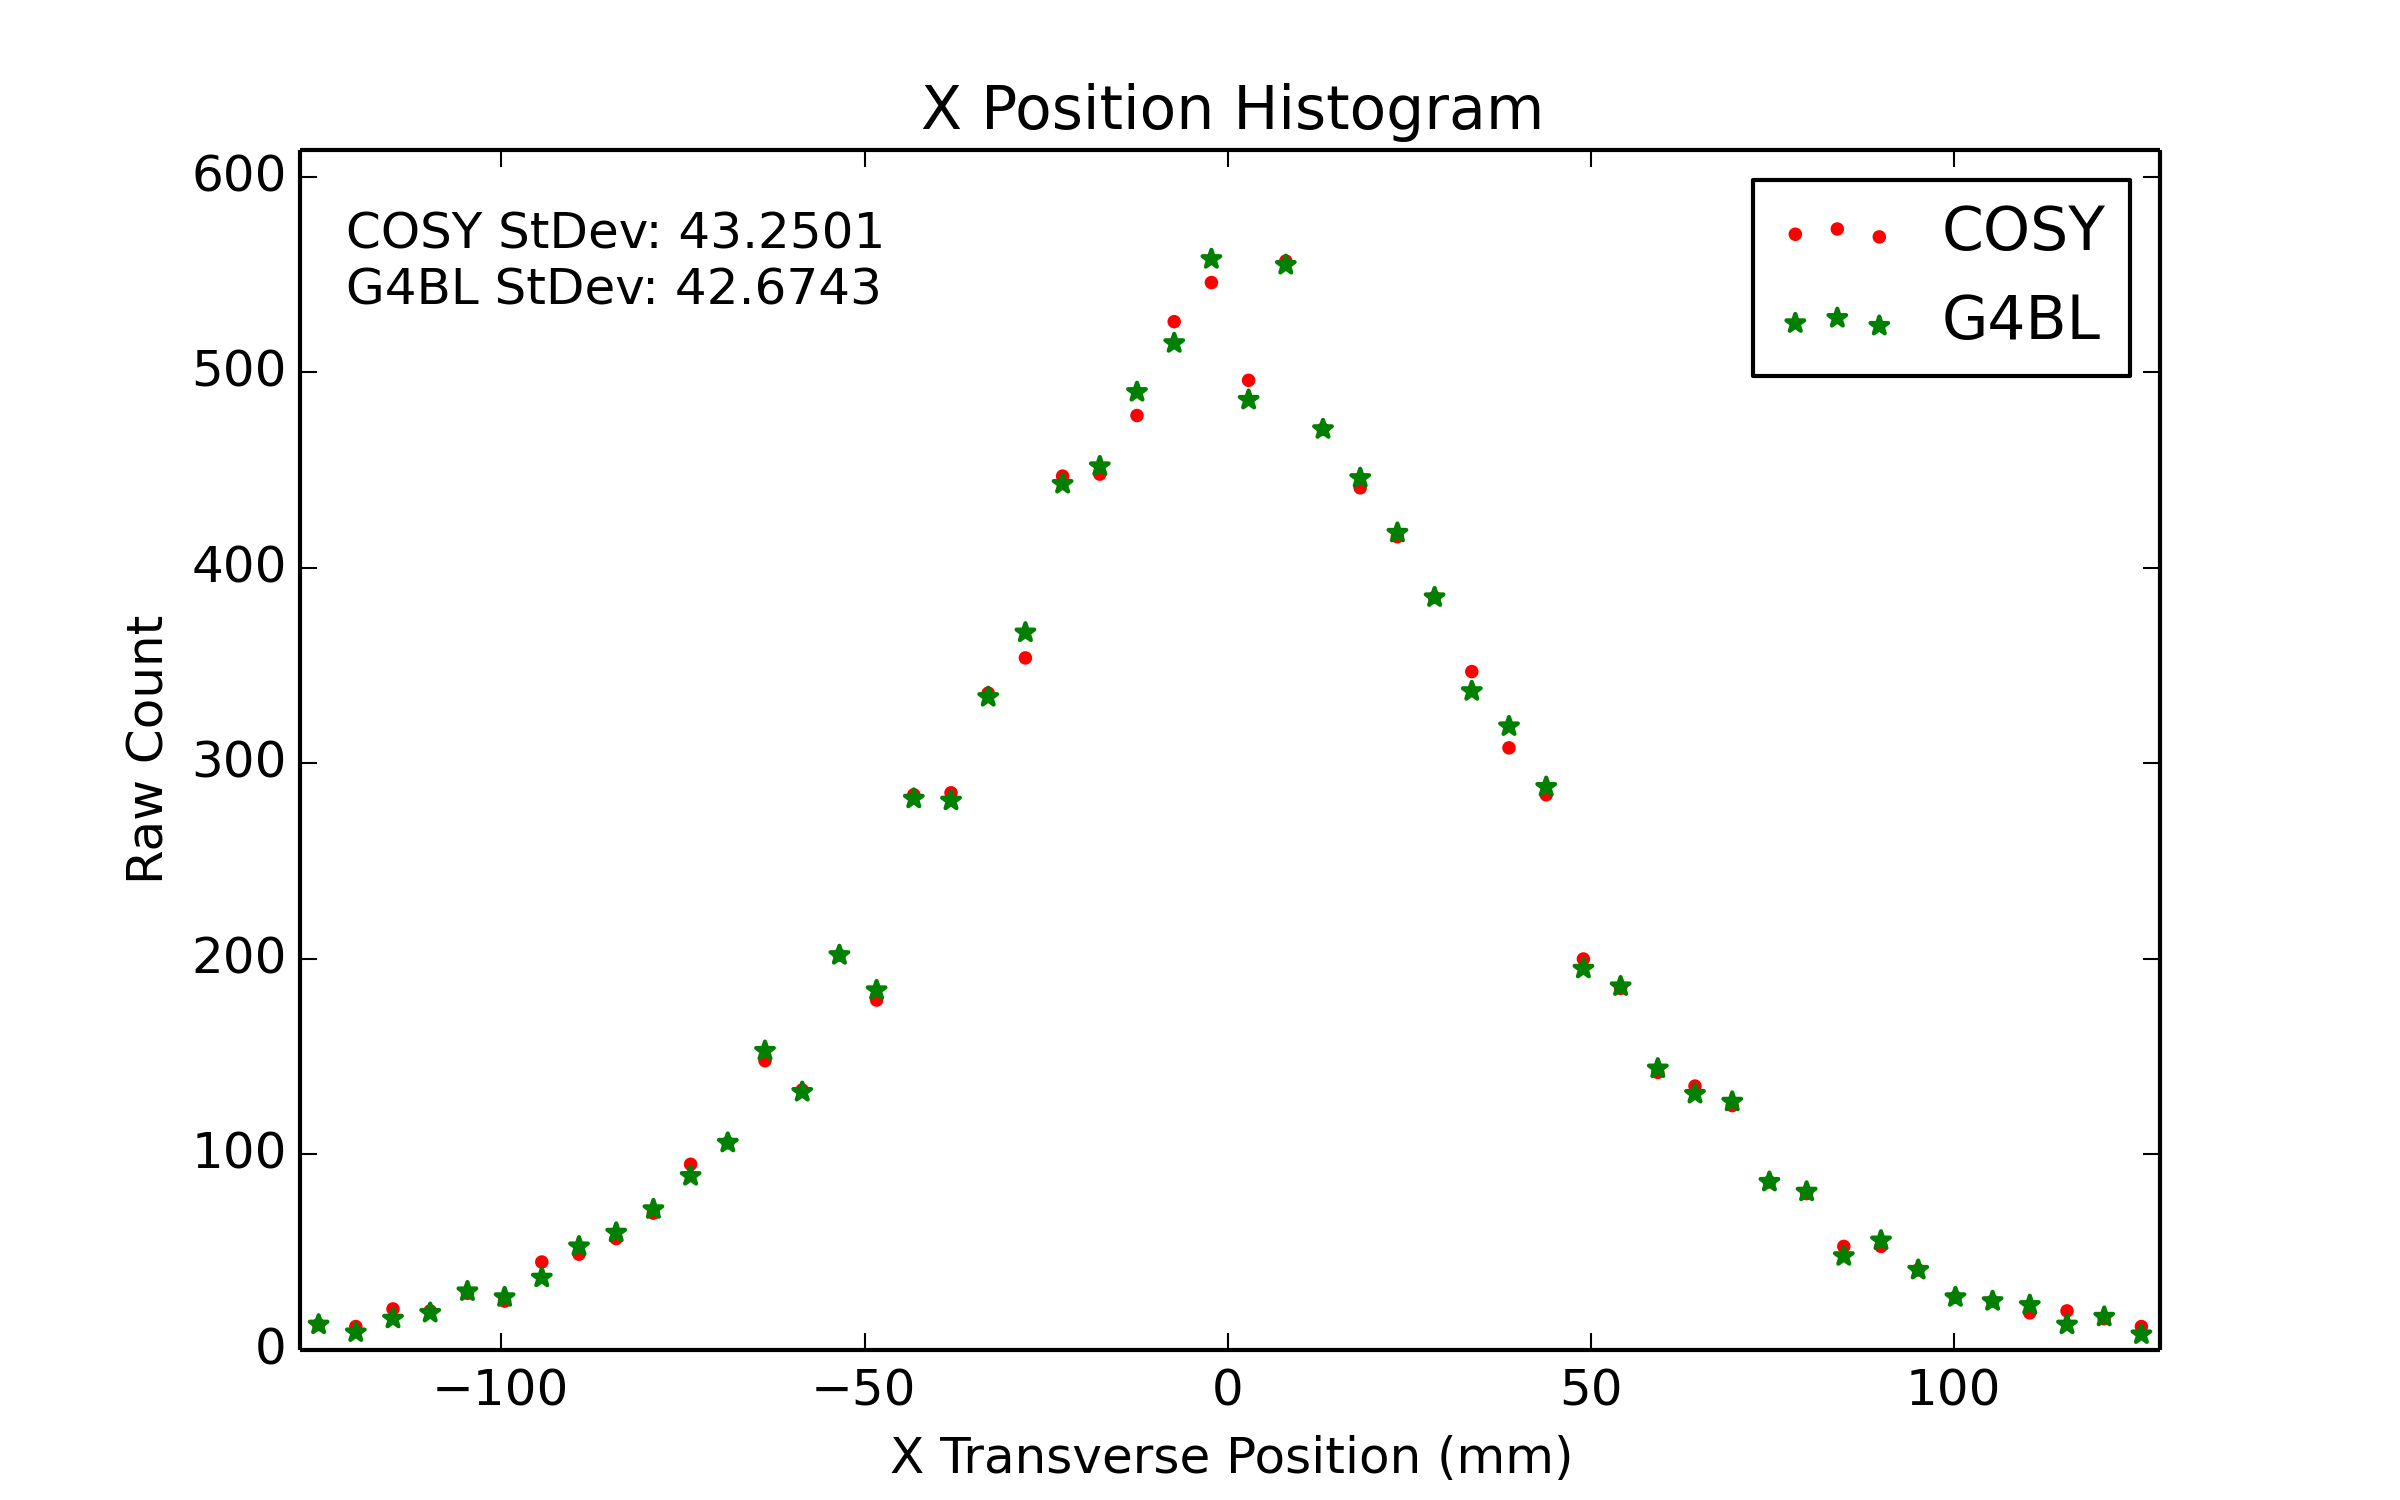
\includegraphics[width=0.5\textwidth]{Figures/coil tests/xposition}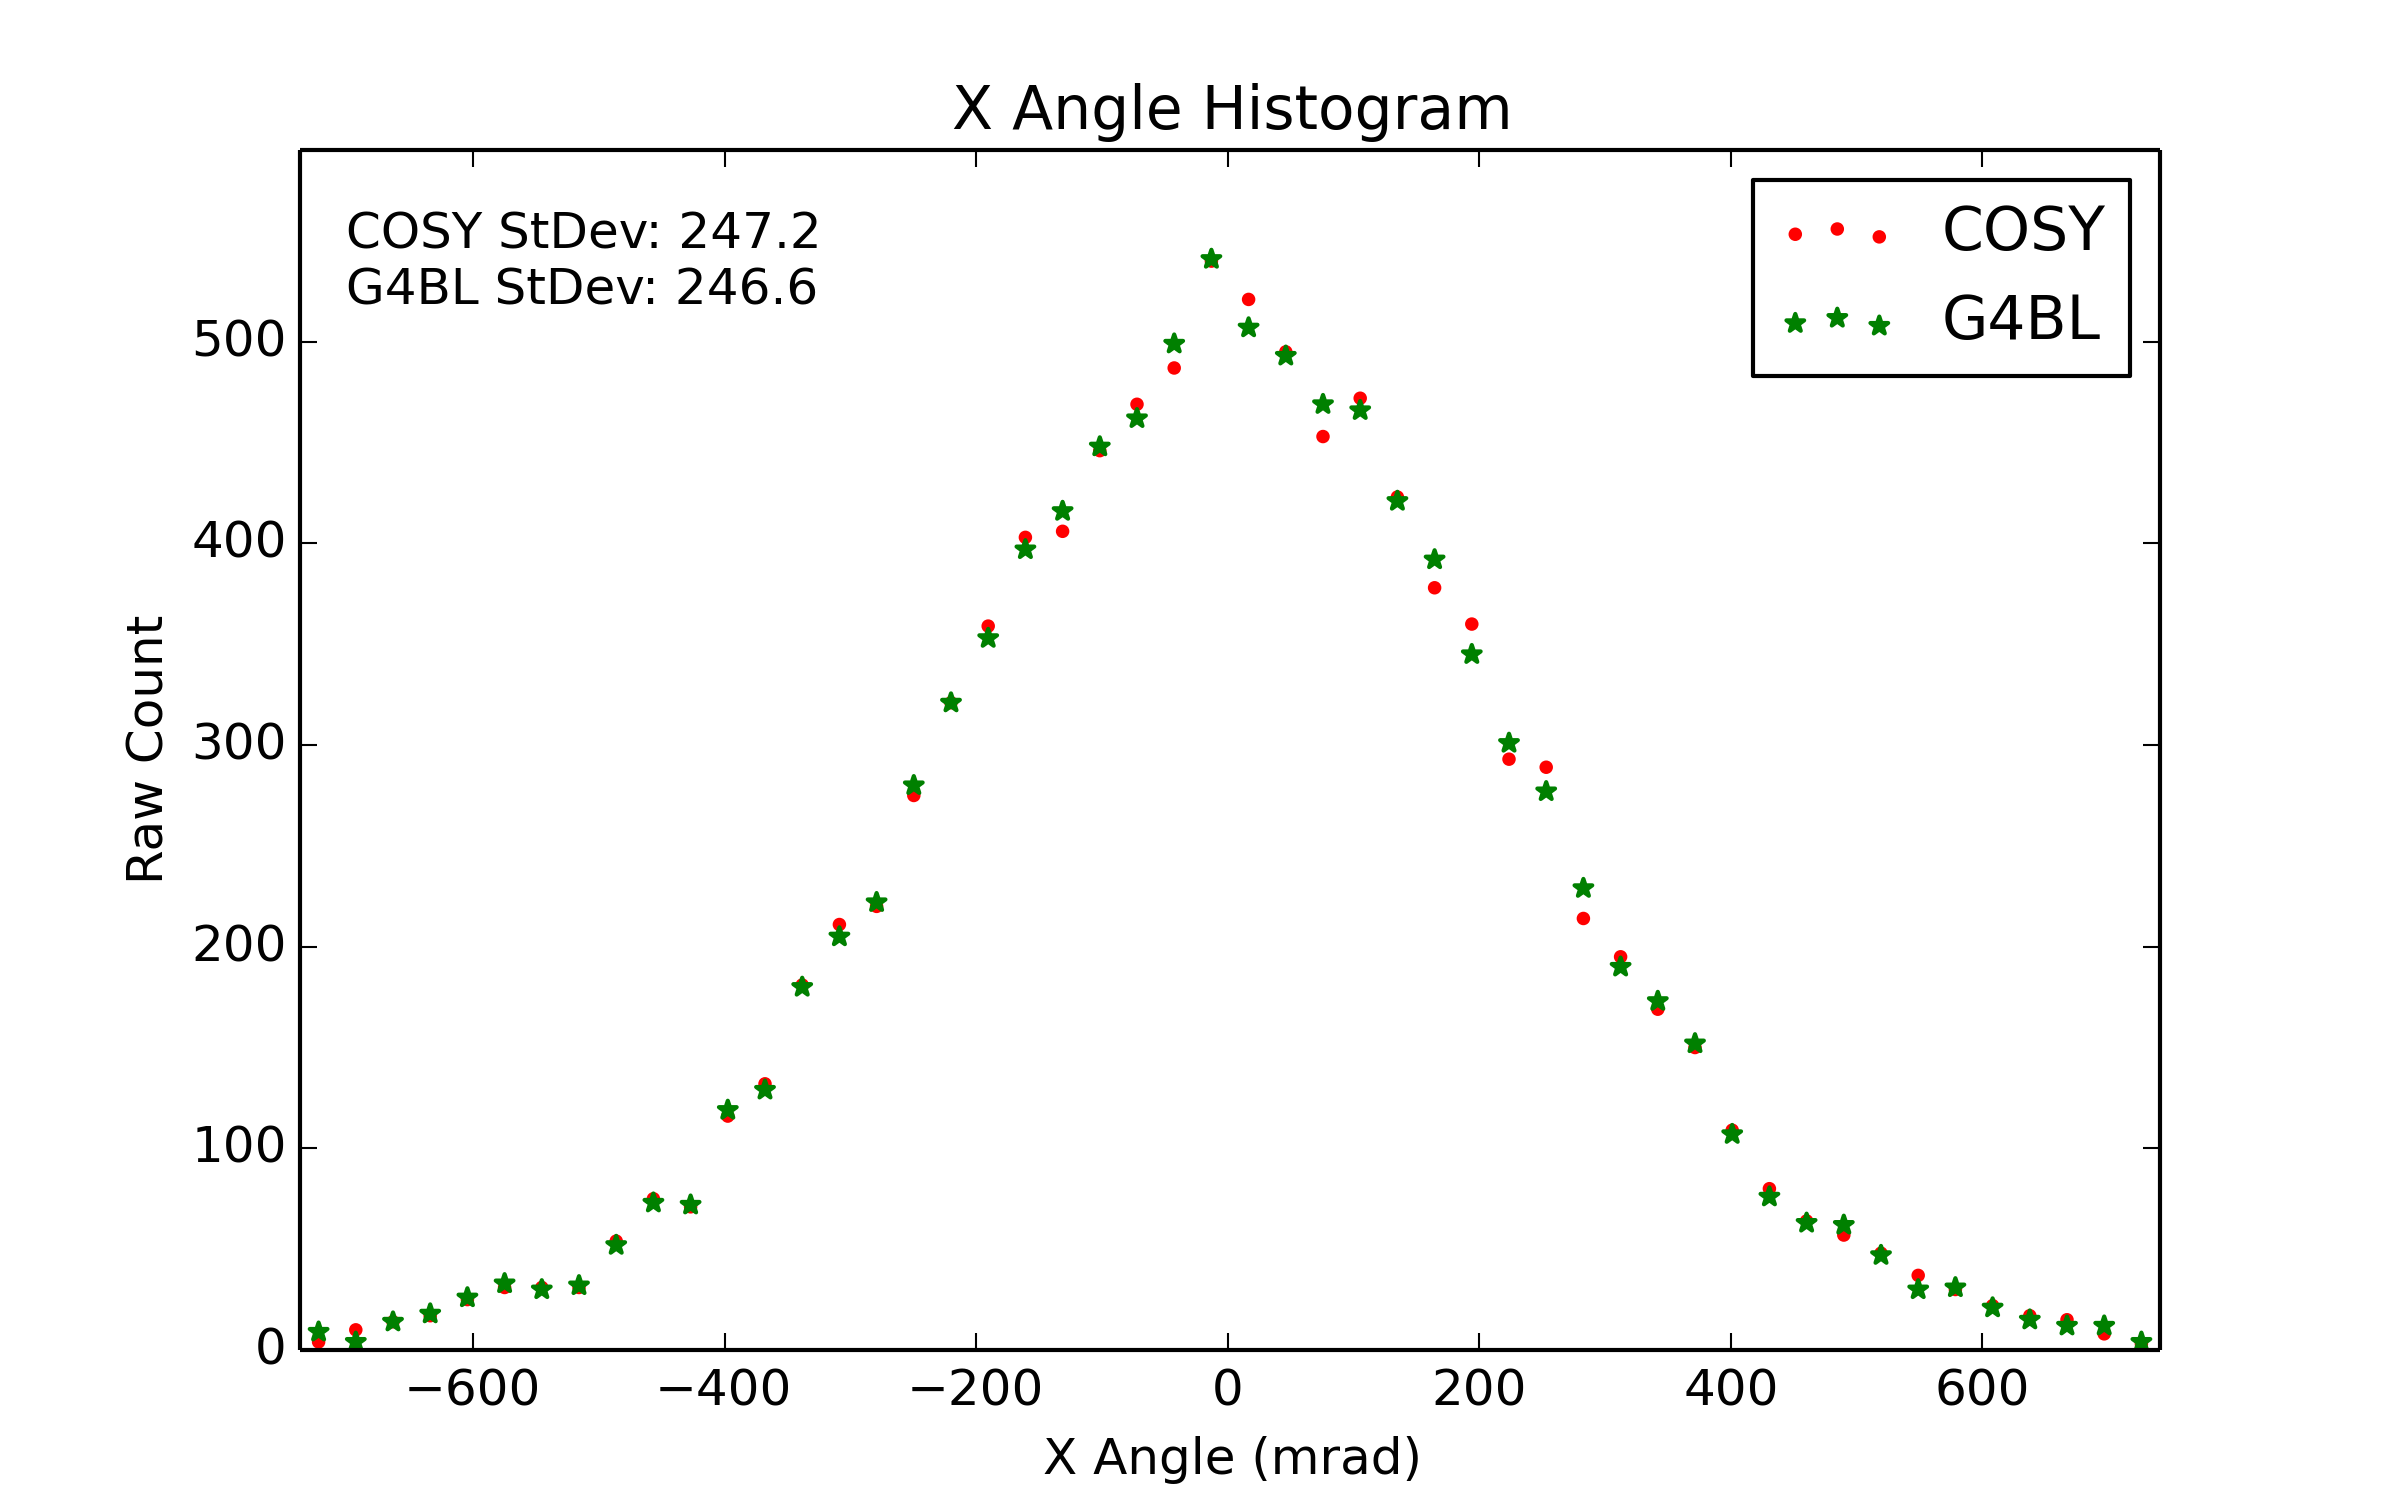
\includegraphics[width=0.5\textwidth]{Figures/coil tests/xangle}
\begin{center} 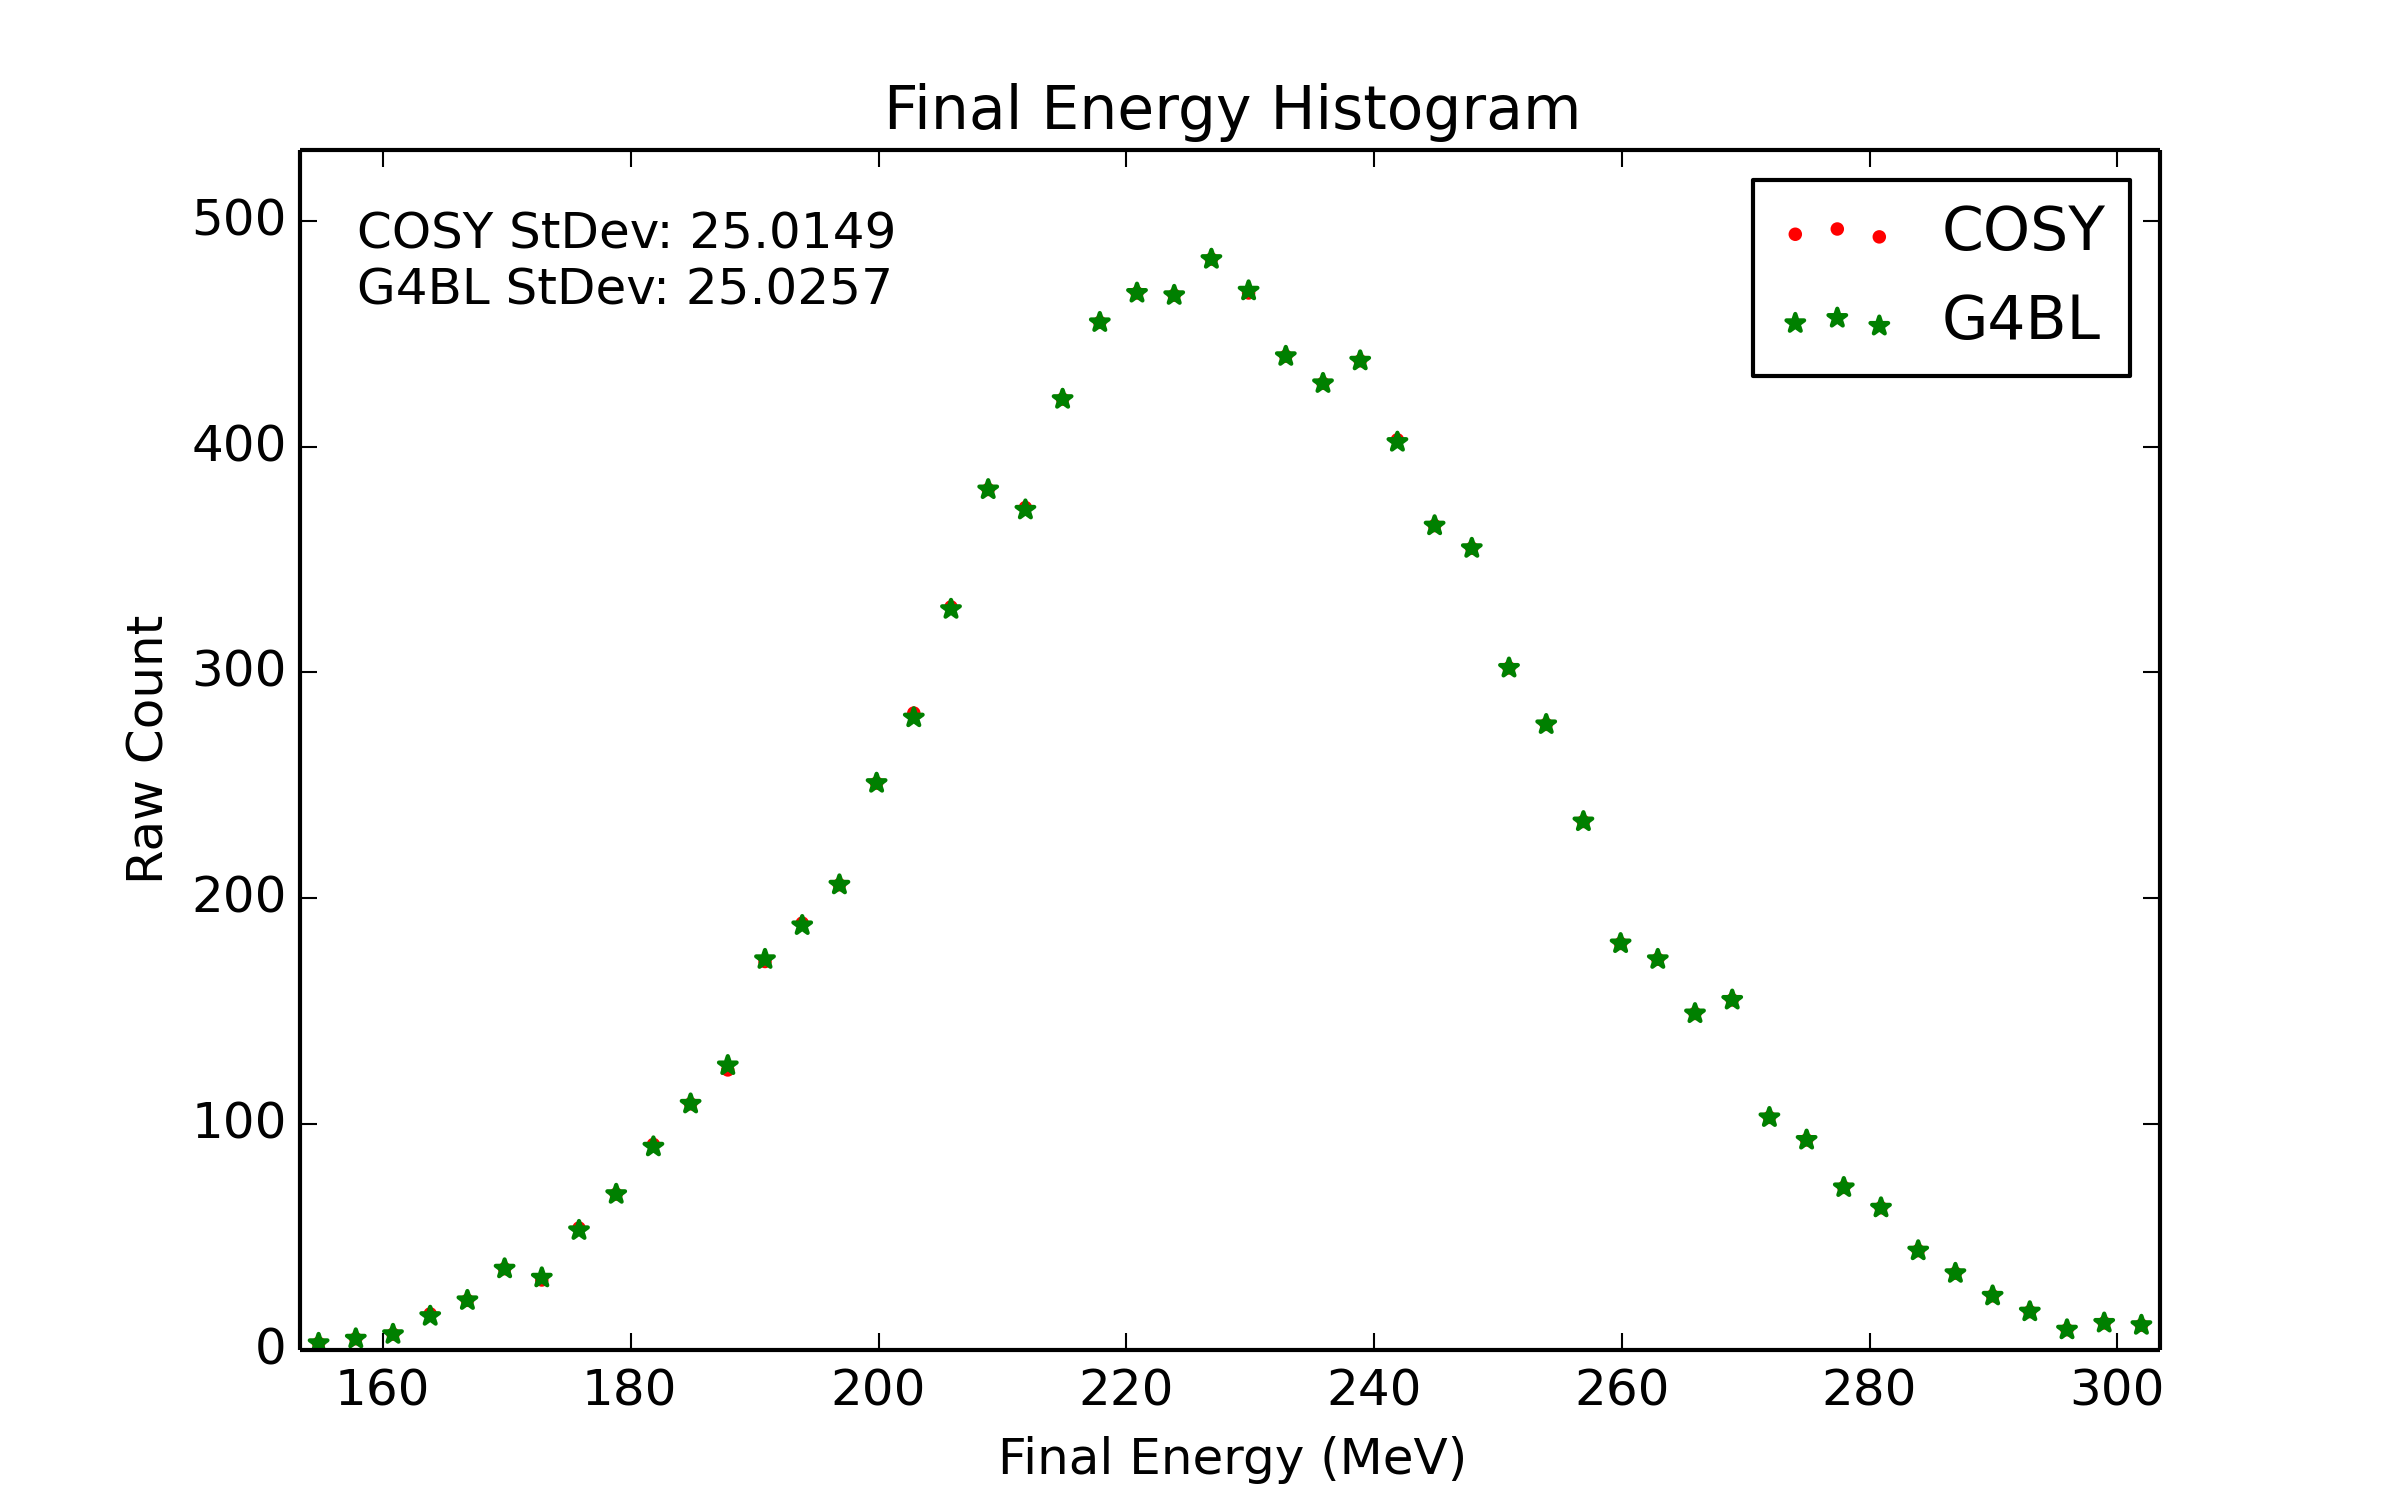
\includegraphics[width=0.5\textwidth]{Figures/coil tests/energy} \end{center}

}

%----------------------------------------------------------------------------------------
%	Current Challenges
%----------------------------------------------------------------------------------------

\headerbox{Current challenges}{name=challenges,column=2,row=1,below=micecell}
{
The details of how to superimpose the absorber and magnetic coils into COSY is still under consideration. Furthermore, a study of tilted coils is desired. In this study, a single cell would consist of four coils tilted about the transverse axis, a wedge absorber, and a radiofrequency cavity. However, a tilted coil routine does not exist in COSY, and so one is desired. Moreover, the differences in the COSY RF kick versus the G4Beamline pillbox model would be explored.
}

%----------------------------------------------------------------------------------------
%	References
%----------------------------------------------------------------------------------------

\headerbox{References}{name=references,column=2,row=2,below=challenges}
{\tiny
\renewcommand{\section}[2]{}% Gets rid of header
\bibliography{bib}{}
\bibliographystyle{unsrt}
}

\end{poster}

\end{document}